\section{Сапёр}
\label{sec:minesweeper}

Напомним вкратце правила игры: необходимо исследовать минное поле, не попав при 
этом ни на одну из них. Минное поле --- это двумерный массив, несколько 
элементов которого содержат скрытые мины, а остальные пусты. В начале игры, 
клетки поля закрыты и игрок должен их исследовать одну за одной. Игрок 
побеждает, если он исследовал все клетки поля, не содержащие мин.

На каждом этапе игры игрок может либо \enq{открыть} клетку либо пометить её как 
\enq{заминированной}. Если он открыл клетку с миной, то игрок проигрывает. 
Иначе клетка меняет свой вид и в ней выводится число заминированных клеток 
вокруг (максимум 8). Если игрок пометил клетку как заминированную, то он не 
может её открыть, не убрав метку.

\begin{figure}[hbt]
	\center{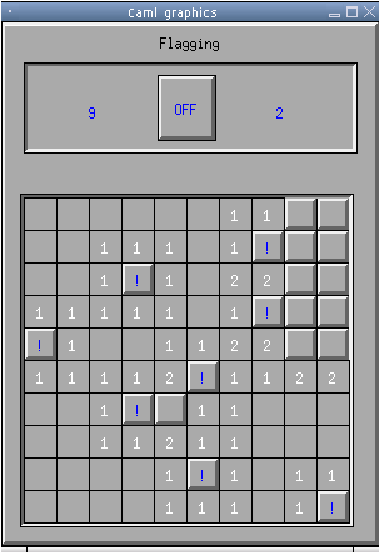
\includegraphics[scale=0.5]{drafts/book012}}
	\caption{\label{fig:screenshot}Снимок экрана}
\end{figure}

Разделим реализацию программы на три части.
\begin{enumerate}
	\item описание абстрактной игры, состоящей из внутреннего представления 
минного поля и функций управляющих этим представлением.

	\item графическое описание игры с соответствующими функциями рисования 
клеток.

	\item часть, отвечающая за взаимодействие между двумя предыдущими частями. 
\end{enumerate}

\subsection{Абстрактное минное поле}
\label{subsec:the_abstract_mine_field}

В этой части мы рассмотрим минное поле как абстрактную сущность, не уделяя 
внимания способам вывода на экран.

\paragraph{Конфигурация}

Минное поле характеризуется своими размерами и числом заминированных клеток. 
Сгруппируем эти три параметра в одной записи и определим конфигурацию по 
умолчанию: размер $10 \times 10$ и $15$ мин.

\begin{lstlisting}[language=OCaml]
# type config = { 
   nbcols  : int ;
   nbrows : int ; 
   nbmines : int };;
# let default_config = { nbcols=10; nbrows=10; nbmines=15 } ;;
\end{lstlisting}

\paragraph{Минное поле}

Вполне естественно будет определить минное поле как двумерный массив. Так же 
нужно уточнить натуру элементов массива и информацию, которую необходимо знать 
для каждого из них. Состояние клетки может быть: 

\begin{itemize}
	\item клетка заминирована?

	\item клетка открыта?

	\item клетка помечена?

	\item сколько из окружающих ячеек заминировано? 
\end{itemize}

Последняя информация не так важна, это значение можно вычислить в нужный момент. 
Но будет проще сделать данный расчёт раз и навсегда в начале игры.

Клетка представлена записью с четырьмя полями, хранящими вышеуказанную 
информацию.

\begin{lstlisting}[language=OCaml]
# type cell = { 
   mutable mined : bool ;
   mutable seen : bool ; 
   mutable flag : bool ; 
   mutable nbm : int
 } ;;
\end{lstlisting}

Двумерный массив есть вектор векторов клеток.

\begin{lstlisting}[language=OCaml]
# type board = cell array array ;;
\end{lstlisting}

\paragraph{Итератор}

Далее в программе нам понадобится применять функцию к каждой клетке поля. 
Реализуем универсальный итератор \code{iter\_cells}, который применяет 
указанную функцию \code{f} к каждому элементу массива конфигурации \code{cf}.

\begin{lstlisting}[language=OCaml]
# let iter_cells cf f = 
   for i=0 to cf.nbcols-1 do for j=0 to cf.nbrows-1 do f (i,j) done done ;;
val iter_cells : config -> (int * int -> 'a) -> unit = <fun>
\end{lstlisting}

Здесь мы получили хорошее сочетание функционального и императивного стилей. Для 
итеративного применения функции с побочным эффектом (она не возвращает 
результат) ко всем элементам массива, используется функция высшего порядка 
(функция, аргумент которой есть другая функция).

\paragraph{Инициализация}

Расположение заминированных клеток будет определяться случайно. Для $r$ и $c$, 
число линий и колонок заминированного поля, и $m$ число мин, необходимо 
получить список состоящий из $m$ чисел в интервале от $1$ до $r * c$. В 
алгоритме подразумевается, что $m < r * c$, однако необходимо сделать эту 
проверку в программе.

Простым решением этой задачи будет создание пустого списка. Затем мы генерируем 
случайное число и размещаем его в список, если оно уже не принадлежит списку. 
Повторим эту операцию до тех пор, пока в списке не будет $m$ чисел. Для этих 
целей, воспользуемся следующими функциями из модулей {\it Random} и {\it Sys}:

\begin{itemize}
	\item \code{Random.int}: \type{int -> int} для входного аргумента $n$ 
возвращает случайное число в диапазоне от $0$ до $n - 1$. 

	\item \code{Random.init}: \type{int -> unit}, инициализация генератора 
случайных чисел.

	\item \code{Sys.time}: \type{unit -> float} возвращает время использования 
процессора в миллисекундах с начала запуска программы. Эта функция используется 
при инициализации генератора случайных чисел при каждой новой игре. 
\end{itemize}

Модули, содержащие эти функции, описаны в главе  \ref{??} на страницах \ref{??} 
и \ref{??} соответственно.

У функции, случайно выбирающей заминированные клетки, два аргумента: общее число 
клеток (\code{cr}) и число мин (\code{m}). Она возвращает список из \code{m} 
линейных координат. 

\begin{lstlisting}[language=OCaml]
# let random_list_mines cr m = 
   let cell_list = ref [] 
   in while (List.length !cell_list) < m do 
        let n = Random.int cr in
         if not (List.mem n !cell_list) then cell_list := n :: !cell_list 
      done ;
     !cell_list ;;
val random_list_mines : int -> int -> int list = <fun>
\end{lstlisting}

Мы не можем заявить что эта функция, так она написана, закончится через 
определённое число итераций. Если генератор случайных чисел достаточно хороший, 
то можно лишь с уверенностью сказать, что вероятность того что эта функция не 
закончится равна нулю. Откуда мы получаем парадоксальное суждение: \enq{функция 
закончится если она выполняется бесконечно}. Однако, на практике эта функция 
никогда нас не подводила, поэтому удовольствуемся данным негарантированным 
определением для генерации списка заминированных клеток.

Для того, чтобы при каждой новой игре получить разные заминированные клетки, 
нужно инициализировать генератор случайных чисел. Инициализировать будем при 
помощи процессорного времени в миллисекундах, которое истекло с момента запуска 
программы.

\begin{lstlisting}[language=OCaml]
# let generate_seed () =
   let t = Sys.time () in
   let n = int_of_float (t*.1000.0) 
   in Random.init(n mod 100000) ;;
val generate_seed : unit -> unit = <fun>
\end{lstlisting}

Практика показывает, что одна и та же программа затрачивает в среднем одинаковое 
время, из–за чего мы получаем схожий результат функции \code{generate\_seed}. В 
связи с этим, функция \code{Unix.time} предпочтительней (см. гл. \ref{??}).

Во время инициализации минного поля, а так же в ходе игры, необходимо знать для 
данной клетки число окружающих заминированных клеток (функция 
\code{neighbors}). При вычислении множества соседних клеток, мы учитываем 
крайние клетки, у которых меньше соседей, чем у тех что находятся в середине 
поля (функция \code{valid}).

\begin{lstlisting}[language=OCaml]
# let valid cf (i,j) = i>=0 && i<cf.nbcols && j>=0 && j<cf.nbrows  ;;
val valid : config -> int * int -> bool = <fun>
# let neighbors cf (x,y) =
   let ngb = [x-1,y-1; x-1,y; x-1,y+1; x,y-1; x,y+1; x+1,y-1; x+1,y; x+1,y+1]
   in List.filter (valid cf) ngb ;;
val neighbors : config -> int * int -> (int * int) list = <fun>
\end{lstlisting}

Инициализация минного поля реализуется функцией \code{initialize\_board}, она 
выполняет четыре задачи:

\begin{enumerate}
	\item генерация списка заминированных клеток

	\item создание двумерного массива состоящего из разных клеток

	\item пометка заминированных клеток

	\item вычисление количества заминированных соседних клеток для каждой 
не заминированной клетки
\end{enumerate}

В этой функции используется несколько локальных функций, которые мы вкратце 
опишем.

\begin{enumerate}
	\item \code{cell\_init}: получить начальные значения клетки.

	\item \code{copy\_cell\_init}: инициализация клетки.

	\item \code{set\_mined}: заминировать клетку.

	\item \code{count\_mined\_adj}: для конкретной клетки вычислить количество 
соседних заминированных клеток.

	\item \code{set\_count}: для конкретной не заминированной клетки обновить 
количество заминированных соседних клеток. 
\end{enumerate}

\begin{lstlisting}[language=OCaml]
# let initialize_board cf = 
   let cell_init () = { mined=false; seen=false; flag=false; nbm=0 } in 
   let copy_cell_init b (i,j) = b.(i).(j) <- cell_init() in
   let set_mined b n = b.(n / cf.nbrows).(n mod cf.nbrows).mined <- true
   in
   let count_mined_adj b (i,j) =
     let x = ref 0 in
     let inc_if_mined (i,j) = if b.(i).(j).mined then incr x 
     in List.iter inc_if_mined (neighbors cf (i,j)) ;
        !x
   in
   let set_count b (i,j) =
     if not b.(i).(j).mined 
     then b.(i).(j).nbm <- count_mined_adj b (i,j)
   in
   let list_mined = random_list_mines (cf.nbcols*cf.nbrows) cf.nbmines in 
   let board = Array.make_matrix cf.nbcols cf.nbrows (cell_init ()) 
   in iter_cells cf (copy_cell_init board) ;
      List.iter (set_mined board) list_mined ;
      iter_cells cf (set_count board) ;
      board ;;
val initialize_board : config -> cell array array = <fun>
\end{lstlisting}

\paragraph{Открытие клетки}

Если во время игры игрок открывает клетку у которой нет ни одного 
заминированного соседа, он с уверенностью может открыть соседние клетки, до тех 
пор пока есть такие клетки. Для того, чтобы избавить игрока от этой нудного 
момента игры, не требующего размышления, игра сама откроет нужные клетки в этом 
случае. При открытии клетки функция \code{cells\_to\_see} возвращает список 
клеток которые можно открыть.

Идея алгоритма достаточно просто излагается: если у открытой клетки есть 
заминированные соседи, то список ограничивается лишь этой самой клеткой, иначе 
список состоит из её соседей, а так же из соседей её соседей. Трудность состоит 
в том, чтобы написать не зацикливающуюся программу, так как клетка является 
соседом самой себе. Надо избежать проверки по несколько раз одной и той же 
клетки поля. Для того, чтобы знать какая клетка была открыта, создадим вектор 
\code{visited} булевых значений. Размер вектора соответствует количеству 
клеток. Если элемент вектора равен \code{true}, это значит что соответствующая 
клетка была исследована. Рекурсивный поиск клеток осуществляется только среди 
не помеченных клеток.

Используя список соседних клеток, функция \code{relevant}, вычисляет два 
под--списка. Каждый под--список состоит из не заминированных, не открытых, не 
помеченных игроком и непроверенных клеток (которым соответствует значение 
\code{false} в векторе \code{visited}, прим. пер.). Первый под--список включает 
соседей, у которых есть как минимум один заминированных сосед, второй состоит 
из соседних клеток без заминированных соседей. Эти клетки помечаются как 
проверенные. Заметим, что помеченные игроком клетки, даже если они на самом 
деле не заминированы, исключаются из списков. Смысл метки заключается как раз в 
том, чтобы избежать открытия клетки.

Функция \code{cells\_to\_see\_rec} рекурсивно реализует цикл поиска. Исходя из 
обновляемого списка клеток, которые необходимо проверить, она возвращает список 
клеток, которые будут открыты. Начальный список содержит лишь последнюю открытую 
клетку, которая помечена как проверенная.

\begin{lstlisting}[language=OCaml]
# let cells_to_see bd cf (i,j) = 
   let visited = Array.make_matrix cf.nbcols cf.nbrows false in 
   let rec relevant = function 
       [] -> ([],[])
     | ((x,y) as c)::t -> 
          let cell=bd.(x).(y)
          in if cell.mined || cell.flag || cell.seen || visited.(x).(y) 
             then relevant t
             else let (l1,l2) = relevant t 
                  in visited.(x).(y) <- true ;
                     if cell.nbm=0 then (l1,c::l2) else (c::l1,l2)
   in 
   let rec cells_to_see_rec = function 
       [] -> []  
     | ((x,y) as c)::t -> 
           if bd.(x).(y).nbm<>0 then c :: (cells_to_see_rec t)
           else let (l1,l2) = relevant (neighbors cf c)
                in  (c :: l1)  @  (cells_to_see_rec (l2 @ t))
   in visited.(i).(j) <- true ;
      cells_to_see_rec [(i,j)]  ;;
val cells_to_see :
  cell array array -> config -> int * int -> (int * int) list = <fun>
\end{lstlisting}

С первого взгляда, аргумент \code{cells\_to\_see\_rec} увеличивается между 
двумя последовательными вызовами функции, тогда как рекуррентное отношение 
основывается на этом аргументе. Соответственно, может возникнуть вопрос --- 
заканчивается ли эта функция? Использование вектора \code{visited} гарантирует, 
что уже проверенная клетка не будет включена в результат \code{relevant}. В то 
же время, клетки, которые добавляются в список проверяемых клеток, происходят 
из \code{relevant}. Этим гарантируется, что определённая клетка будет 
возвращена \code{relevant} всего один раз и в следствии она будет представлена 
в единственном экземпляре в списке проверяемых клеток. Раз количество клеток 
ограничено, значит наша функция тоже закончится.

На этом неграфическая часть игры заканчивается. Рассмотрим стиль 
программирования, которым мы воспользовались. Выбор изменяемых структур данных 
вынуждает использовать императивный стиль с циклами и присвоением. Однако, для 
решения дополнительных задач мы применили списки и функции обработки в 
функциональном стиле. Стиль программирования предписывается структурами данных, 
которыми мы манипулируем. Функция \code{cells\_to\_see} тому хороший пример: 
она использует списки и, вполне естественно, эта функция написана в 
функциональном стиле. Для хранения информации о проверенных клетках мы 
используем вектор, обновление вектора осуществляется императивно. Конечно, мы 
могли бы сделать тоже самое в чисто функциональном стиле, используя список. 
Однако, цена этого решения выше, чем для предыдущего (поиск элемента в списке 
напрямую зависит от размера списка, тогда как для вектора время поиск есть 
константная величина) и оно не является более простым.

\subsection{Игровой интерфейс}
\label{subsec:displaying_the_minesweeper_game}

Эта часть игры зависит от структур данных, которые представляют состояние игры 
(см. \ref{subsec:the_abstract_mine_field}). Цель этой части --- изобразить на 
экране различные компоненты игры, как на рисунке 
\ref{fig:the_main_window_of_minesweeper}. Для этого воспользуемся функциями 
рисования блоков, описанными ранее на 
\ref{subsec:example_drawing_of_boxes_with_relief_patterns}.

\begin{figure}[h]
	\center{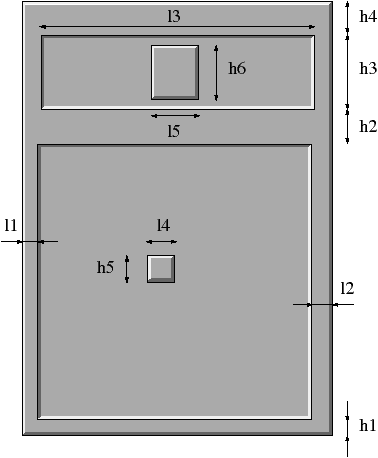
\includegraphics[scale=0.5]{drafts/book013}}
	\caption{\label{fig:the_main_window_of_minesweeper}Основное окно игры}
\end{figure}

Свойства различных компонентов игры описываются следующими параметрами. 

\begin{table}[hl]
\begin{center}
	\label{tbl:operations_on_numbers}
	\caption{Операции над числами}
	\begin{tabular}{|p{7.2cm}|p{7.2cm}|}
	\hline
{\begin{lstlisting}[language=OCaml,frame=none]
# let b0 = 3 ;;
# let w1 = 15 ;;
# let w2 = w1 ;;
# let w4 = 20 + 2*b0 ;;
# let w3 = w4*default_config.nbcols + 2*b0 ;;
# let w5 = 40 + 2*b0 ;;
\end{lstlisting}}
 &
{\begin{lstlisting}[language=OCaml,frame=none]
# let h1 = w1 ;;
# let h2 = 30 ;;
# let h3 = w5+20 + 2*b0 ;;
# let h4 = h2 ;;
# let h5 = 20 + 2*b0 ;;
# let h6 = w5 + 2*b0 ;;
\end{lstlisting}}
\\
	\hline
	\end{tabular}
\end{center}
\end{table}

При помощи этих параметров мы расширим базовую конфигурацию игры (значения с 
типом \code{config}) и определим новую запись \code{window\_config}. В поле 
\code{cf} содержится минимальная конфигурация. Каждой компоненте, изображённой 
на экране, ассоциируем блок: основное окно (поле \code{main\_box}), минное поле 
(поле \code{field\_box}), диалоговое окно (поле \code{dialog\_box}) из двух 
блоков (поля \code{d1\_box} и \code{d2\_box}), кнопка для пометки (поле 
\code{flag\_box}) и текущая клетка (поле \code{current\_box}).

\begin{lstlisting}[language=OCaml]
# type window_config = {
   cf : config ;
   main_box : box_config ;
   field_box : box_config ;
   dialog_box : box_config ;
   d1_box : box_config ;
   d2_box : box_config ;
   flag_box : box_config ;
   mutable current_box : box_config ;
   cell : int*int -> (int*int) ;
   coor : int*int -> (int*int)
 } ;;
\end{lstlisting}

Кроме этого, значение с типом \code{window\_config} содержит две функции:

\begin{itemize}
	\item \code{cell}: для координат данной клетки возвращает координаты её 
блока

	\item \code{coor}: для координат пикселя окна возвращает координаты 
соответствующей клетки.
\end{itemize}

\paragraph{Конфигурация}

Определим функцию, которая создаёт графическую конфигурацию (с типом 
\code{window\_config}) в соответствии с минимальной конфигурацией (с типом 
\code{config}) и вышеописанных параметров. Значения параметров некоторых 
компонент зависят друг от друга. Например, ширина основного блока зависит от 
ширины блока минного поля, которых в свою очередь зависит от количества 
столбцов. Чтобы не вычислять одно и то же по несколько раз, мы будем постепенно 
инициализировать эти поля. В отсутствии специальных функций данный этап 
инициализации немного нудный.

\begin{lstlisting}[language=OCaml]
# let make_box x y w h bw r =
   { x=x; y=y; w=w; h=h; bw=bw; r=r; b1_col=gray1; b2_col=gray3; b_col=gray2 } 
;;
val make_box : int -> int -> int -> int -> int -> relief -> box_config =
  <fun>
# let make_wcf cf = 
   let wcols =  b0 + cf.nbcols*w4 + b0 
   and hrows =  b0 + cf.nbrows*h5 + b0  in
   let main_box =  let gw = (b0 + w1 + wcols + w2 + b0) 
                and gh = (b0 + h1 + hrows + h2 + h3 + h4 + b0)
                in make_box 0 0 gw gh b0 Top
   and field_box = make_box w1 h1 wcols hrows b0 Bot  in
   let dialog_box = make_box  ((main_box.w - w3) / 2)
                              (b0+h1+hrows+h2)
                              w3 h3 b0 Bot
   in 
   let d1_box = make_box (dialog_box.x + b0) (b0 + h1 + hrows + h2)
                         ((w3-w5)/2-(2*b0)) (h3-(2*b0)) 5 Flat  in
   let flag_box = make_box (d1_box.x + d1_box.w) 
                        (d1_box.y + (h3-h6) / 2) w5 h6 b0 Top  in 
   let d2_box = make_box (flag_box.x + flag_box.w) 
                         d1_box.y d1_box.w d1_box.h 5 Flat  in
   let current_box = make_box 0 0 w4 h5 b0 Top
   in { cf = cf; 
        main_box = main_box; field_box=field_box; dialog_box=dialog_box;
        d1_box=d1_box; 
        flag_box=flag_box; d2_box=d2_box; current_box = current_box;
        cell = (fun (i,j) -> ( w1+b0+w4*i , h1+b0+h5*j)) ;
        coor = (fun (x,y) -> ( (x-w1)/w4 , (y-h1)/h5 )) } ;;
val make_wcf : config -> window_config = <fun>
\end{lstlisting}

\paragraph{Вывод клеток}

Теперь нам предстоит определить функции вывода клеток в различных случаях: 
клетка может быть открыта или закрыта, содержать или нет информацию. Вывод 
(блока) текущей клетки всегда будет осуществляться (поле \code{cc\_bcf}).

Определим две функции изменяющие конфигурацию текущей клетки; одна закрывает 
клетку, другая открывает её.

\begin{lstlisting}[language=OCaml]
# let close_ccell wcf i j =
   let x,y = wcf.cell (i,j)
   in wcf.current_box <- {wcf.current_box with x=x; y=y; r=Top} ;;
val close_ccell : window_config -> int -> int -> unit = <fun>
# let open_ccell wcf i j =
   let x,y = wcf.cell (i,j)
   in wcf.current_box <- {wcf.current_box with x=x; y=y; r=Flat} ;;
val open_ccell : window_config -> int -> int -> unit = <fun>
\end{lstlisting}

В зависимости от ситуации, необходимо выводить информацию на клетках. Для 
каждого случая мы определяем функцию.

\begin{itemize}
	\item Вывод закрытой клетки:

\begin{lstlisting}[language=OCaml]
# let draw_closed_cc wcf i j =
  close_ccell wcf i j;
  draw_box wcf.current_box ;;
val draw_closed_cc : window_config -> int -> int -> unit = <fun>
\end{lstlisting}

	\item Вывести открытую клетку с числом мин:

\begin{lstlisting}[language=OCaml]
# let draw_num_cc wcf i j n =
   open_ccell wcf i j ;
   draw_box wcf.current_box ;
   if n<>0 then draw_string_in_box Center (string_of_int n) 
                                   wcf.current_box Graphics.white ;;
val draw_num_cc : window_config -> int -> int -> int -> unit = <fun>
\end{lstlisting}

	\item Вывод клетки, содержащей мину:

\begin{lstlisting}[language=OCaml]
# let draw_mine_cc wcf i j = 
   open_ccell wcf i j ;
   let cc = wcf.current_box 
   in draw_box wcf.current_box ;
      Graphics.set_color Graphics.black ; 
      Graphics.fill_circle (cc.x+cc.w/2) (cc.y+cc.h/2) (cc.h/3) ;;
val draw_mine_cc : window_config -> int -> int -> unit = <fun>
\end{lstlisting}

	\item Вывод заминированной и помеченной клетки:

\begin{lstlisting}[language=OCaml]
# let draw_flag_cc wcf i j =
   close_ccell wcf i j ;
   draw_box wcf.current_box ;
   draw_string_in_box Center "!" wcf.current_box Graphics.blue ;;
val draw_flag_cc : window_config -> int -> int -> unit = <fun>
\end{lstlisting}

	\item Вывод ошибочно помеченной клетки: 

\begin{lstlisting}[language=OCaml]
# let draw_cross_cc wcf i j =
  let x,y = wcf.cell (i,j)
  and w,h = wcf.current_box.w, wcf.current_box.h in
  let a=x+w/4 and b=x+3*w/4 
  and c=y+h/4 and d=y+3*h/4 
  in Graphics.set_color Graphics.red ;
     Graphics.set_line_width 3 ;
     Graphics.moveto a d ; Graphics.lineto b c ;
     Graphics.moveto a c ; Graphics.lineto b d ;
     Graphics.set_line_width 1 ;;
val draw_cross_cc : window_config -> int -> int -> unit = <fun>
\end{lstlisting}

\end{itemize}

В ходе игры, выбор соответствующей функции вывода клетки осуществляется 
следующим:

\begin{lstlisting}[language=OCaml]
# let draw_cell wcf bd i j =
   let cell = bd.(i).(j)
   in match (cell.flag, cell.seen , cell.mined ) with
          (true,_,_)  -> draw_flag_cc wcf i j
        | (_,false,_) -> draw_closed_cc wcf i j
        | (_,_,true)  -> draw_mine_cc wcf i j
        | _           -> draw_num_cc wcf i j cell.nbm  ;;
val draw_cell : window_config -> cell array array -> int -> int -> unit =
  <fun>
\end{lstlisting}

Для вывода клеток в конце игры, воспользуемся специальной функцией. Она немного 
отличается от предыдущих тем, что к концу все клетки должны быть открыты. К тому 
же, на ошибочно помеченных клетках выводится красный крест.

\begin{lstlisting}[language=OCaml]
# let draw_cell_end wcf bd i j =
   let cell = bd.(i).(j)
   in match (cell.flag, cell.mined ) with
          (true,true) -> draw_flag_cc wcf i j
        | (true,false) -> draw_num_cc wcf i j cell.nbm; draw_cross_cc wcf i j
        | (false,true) -> draw_mine_cc wcf i j
        | (false,false) -> draw_num_cc wcf i j cell.nbm ;;
val draw_cell_end : window_config -> cell array array -> int -> int -> unit =
  <fun>
\end{lstlisting}

\paragraph{Вывод остальных компонентов}

Состояние режима отметки клеток отображается выпуклым или вогнутым блоком с 
надписью \code{ON} или \code{OFF}:

\begin{lstlisting}[language=OCaml]
# let draw_flag_switch wcf on =
   if on  then wcf.flag_box.r <- Bot  else wcf.flag_box.r <- Top ;
   draw_box wcf.flag_box ;
   if on  then draw_string_in_box Center "ON" wcf.flag_box Graphics.red
   else draw_string_in_box Center "OFF" wcf.flag_box Graphics.blue ;;
val draw_flag_switch : window_config -> bool -> unit = <fun>
\end{lstlisting}

Выведем надпись о предназначении помечающей кнопки.

\begin{lstlisting}[language=OCaml]
# let draw_flag_title wcf =
   let m = "Flagging" in
   let w,h = Graphics.text_size m in
   let x = (wcf.main_box.w-w)/2
   and y0 = wcf.dialog_box.y+wcf.dialog_box.h in
   let y = y0+(wcf.main_box.h-(y0+h))/2 
   in Graphics.moveto x y ;
      Graphics.draw_string m ;;
val draw_flag_title : window_config -> unit = <fun>
\end{lstlisting}

На протяжении всей игры число клеток, которые осталось открыть и число
помеченных клеток выводится в диалоговом окне с обеих сторон помечающей кнопки.

\begin{lstlisting}[language=OCaml]
# let print_score wcf nbcto nbfc =
   erase_box wcf.d1_box ;
   draw_string_in_box Center (string_of_int nbcto) wcf.d1_box Graphics.blue ;
   erase_box wcf.d2_box ;
   draw_string_in_box Center (string_of_int (wcf.cf.nbmines-nbfc)) wcf.d2_box 
    ( if nbfc>wcf.cf.nbmines then Graphics.red else Graphics.blue ) ;;
val print_score : window_config -> int -> int -> unit = <fun>
\end{lstlisting}

Чтобы нарисовать начальное минное поле, нужно вывести (число линий) $\times$ 
(число столбцов) раз закрытую клетку. Хоть это и один и тот же рисунок каждый 
раз необходимо нарисовать и заполнить прямоугольный и четыре трапеции, на это 
может уйти немало времени. Для ускорения этого процесса, воспользуемся 
следующей техникой: нарисуем один раз клетку, захватим её в виде растрового 
изображения и затем скопируем эту кнопку в нужных местах.

\begin{lstlisting}[language=OCaml]
# let draw_field_initial wcf =
   draw_closed_cc wcf 0 0 ;
   let cc = wcf.current_box  in
   let bitmap = draw_box cc ; Graphics.get_image cc.x cc.y cc.w cc.h  in
   let draw_bitmap (i,j) = let x,y=wcf.cell (i,j)
                           in Graphics.draw_image bitmap x y 
   in iter_cells wcf.cf draw_bitmap  ;;
val draw_field_initial : window_config -> unit = <fun>
\end{lstlisting}

В конце игры, все минное поле открывается и на неправильно помеченных клетках 
ставится красный крест.

\begin{lstlisting}[language=OCaml]
# let draw_field_end wcf bd = 
   iter_cells wcf.cf (fun (i,j) -> draw_cell_end wcf bd i j)  ;;
val draw_field_end : window_config -> cell array array -> unit = <fun>
\end{lstlisting}

И наконец, основная функция вывода на экран открывает графический контекст и 
выводит начальное состояние различных компонент.

\begin{lstlisting}[language=OCaml]
# let open_wcf wcf =
   Graphics.open_graph ( " " ^ (string_of_int wcf.main_box.w) ^ "x" ^
                         (string_of_int wcf.main_box.h)               ) ;
   draw_box wcf.main_box ;
   draw_box wcf.dialog_box ;
   draw_flag_switch wcf false ;
   draw_box wcf.field_box ;
   draw_field_initial wcf ;
   draw_flag_title wcf ;
   print_score wcf ((wcf.cf.nbrows*wcf.cf.nbcols)-wcf.cf.nbmines) 0 ;;
val open_wcf : window_config -> unit = <fun>
\end{lstlisting}

Заметим, что все графические функции используют конфигурацию с типом
\code{window\_config}. Это делает их независимыми от расположения компонент 
игры. Если мы пожелаем изменить это расположение, код функций останется 
неизменным, необходимо будет лишь обновить конфигурацию.

\subsection{Взаимодействие между программой и игроком}
\label{subsec:interaction_with_the_player}

Определим возможные действия игрока:

\begin{itemize}
	\item выбрать, нажатием кнопки, режим пометки или открытия клетки. 

	\item нажать на одну из клеток, для того чтобы ее открыть или пометить. 

	\item нажать на клавишу 'q', для того чтобы покинуть игру. 
\end{itemize}

Напомним, что событие \code{Graphics} должно быть связанно с записью 
(\code{Graphics.status}), в которой хранится информация о текущем состоянии 
клавиатуры и мыши в момент возникновения события. Все события мыши, кроме 
нажатия на кнопку пометки или на клетку минного поля, игнорируются. Чтобы 
различать оба события, создадим соответствующий тип.

\begin{lstlisting}[language=OCaml]
# type clickon = Out | Cell of (int*int) | SelectBox  ;;
\end{lstlisting}

Действия нажатия и отпускания кнопки мыши соответствуют двум разным событиям. 
Если оба события произошли на одной и той же компоненте (клетка минного поля или 
кнопка пометки), то такой клик считается правильным о обрабатывается.

\begin{lstlisting}[language=OCaml]
# let locate_click wcf st1 st2 =
   let clickon_of st = 
     let x = st.Graphics.mouse_x and y = st.Graphics.mouse_y
     in if x>=wcf.flag_box.x && x<=wcf.flag_box.x+wcf.flag_box.w && 
           y>=wcf.flag_box.y && y<=wcf.flag_box.y+wcf.flag_box.h  
        then SelectBox
        else let (x2,y2) = wcf.coor (x,y)
             in if x2>=0 && x2<wcf.cf.nbcols && y2>=0 && y2<wcf.cf.nbrows
                then Cell (x2,y2) else Out
   in 
   let r1=clickon_of st1 and r2=clickon_of st2
   in if r1=r2 then r1 else Out ;;
val locate_click :
  window_config -> Graphics.status -> Graphics.status -> clickon = <fun>
\end{lstlisting}

Сердце программы находится в функции \code{loop} и заключается в ожидании и
обработке событий. Эта функция похожа на \code{skel}, описанной на 
\ref{subsec:program_skeleton}, однако здесь мы точнее определяем тип события 
мыши. Условия остановки цикла следующие:

\begin{itemize}
	\item нажатие на клавишу q (или Q), что рассматривается как желание 
остановить программу.

	\item в случае если игрок открыл заминированную клетку, тогда партия 
проиграна.

	\item в случае если игрок открыл все незаминированные клетки, тогда партия. 
выиграна.
\end{itemize}

Объединим данные, необходимые функциям обрабатывающим взаимодействие с игроком, 
в записи \code{minesw\_cf}.

\begin{lstlisting}[language=OCaml]
# type minesw_cf =
   { wcf : window_config; bd : cell array array;
     mutable nb_flagged_cells : int;
     mutable nb_hidden_cells : int;
     mutable flag_switch_on : bool } ;;
\end{lstlisting}

Эти поля соответствуют:

\begin{itemize}
	\item \code{wcf}: графическая конфигурация.

	\item \code{bd}: матрица клеток.

	\item \code{nb\_flagged\_cells}: булево значение, означающее что игра
находится или нет в режиме пометки.

	\item \code{nb\_hidden\_cells}: число помеченных клеток

	\item \code{flag\_switch\_on}: число незаминированных и неоткрытых клеток 
\end{itemize}

Теперь мы готовы, к тому чтобы написать основной цикл.

\begin{lstlisting}[language=OCaml]
# let loop d f_init f_key f_mouse f_end = 
   f_init ();
   try
     while true do 
       let st = Graphics.wait_next_event 
                  [Graphics.Button_down;Graphics.Key_pressed]  
       in if st.Graphics.keypressed  then f_key st.Graphics.key
          else let st2 = Graphics.wait_next_event [Graphics.Button_up] 
               in f_mouse (locate_click d.wcf st st2)
     done
   with End -> f_end ();;
val loop :
  minesw_cf ->
  (unit -> 'a) -> (char -> 'b) -> (clickon -> 'b) -> (unit -> unit) -> unit =
  <fun>
\end{lstlisting}

Функции инициализации, окончания и обработки клавиатуры достаточно банальны.

\begin{lstlisting}[language=OCaml]
# let d_init d () = open_wcf d.wcf
 let d_end  () = Graphics.close_graph()
 let d_key c = if c='q' || c='Q' then raise End;;
val d_init : minesw_cf -> unit -> unit = <fun>
val d_end : unit -> unit = <fun>
val d_key : char -> unit = <fun>
\end{lstlisting}

Для обработки событий мыши нам понадобится несколько дополнительных функций.


\begin{itemize}
	\item \code{flag\_cell}: реакция на клик на клетку в режиме пометки.

	\item \code{ending}: конец игры. В этом случае открыть все заминированные 
клетки, вывести сообщение о победе или проигрыше и ожидать действия с клавиатуры 
или мыши для того, чтобы закрыть программу.

	\item \code{reveal}: реакция на клик на клетку в режиме открытия (режим 
пометки отключен).
\end{itemize}

\begin{lstlisting}[language=OCaml]
# let flag_cell d i j =
   if d.bd.(i).(j).flag 
   then ( d.nb_flagged_cells <- d.nb_flagged_cells -1; 
          d.bd.(i).(j).flag <- false )
   else ( d.nb_flagged_cells <- d.nb_flagged_cells +1; 
          d.bd.(i).(j).flag <- true );
   draw_cell d.wcf d.bd i j;
   print_score d.wcf d.nb_hidden_cells d.nb_flagged_cells;;
val flag_cell : minesw_cf -> int -> int -> unit = <fun>

# let ending d str = 
   draw_field_end d.wcf d.bd;
   erase_box  d.wcf.flag_box;
   draw_string_in_box Center str d.wcf.flag_box Graphics.black;
   ignore(Graphics.wait_next_event 
            [Graphics.Button_down;Graphics.Key_pressed]);
   raise End;;
val ending : minesw_cf -> string -> 'a = <fun>

# let reveal d i j = 
   let reveal_cell (i,j) = 
     d.bd.(i).(j).seen <- true; 
     draw_cell d.wcf d.bd i j;
     d.nb_hidden_cells <- d.nb_hidden_cells -1 
   in 
     List.iter reveal_cell (cells_to_see d.bd d.wcf.cf (i,j));
     print_score d.wcf d.nb_hidden_cells d.nb_flagged_cells;
     if d.nb_hidden_cells = 0 then ending d "WON";;
val reveal : minesw_cf -> int -> int -> unit = <fun>
\end{lstlisting}

Функция, обрабатывающая события мыши, сопоставляет значение типа \code{clickon}.

\begin{lstlisting}[language=OCaml]
# let d_mouse d click = match click with
     Cell (i,j) ->
       if d.bd.(i).(j).seen then ()
       else if d.flag_switch_on then flag_cell d i j 
       else if d.bd.(i).(j).flag then ()
       else if d.bd.(i).(j).mined then ending d "LOST"
       else reveal d i j
   | SelectBox ->
       d.flag_switch_on <- not d.flag_switch_on;
       draw_flag_switch d.wcf d.flag_switch_on
   | Out -> () ;;
val d_mouse : minesw_cf -> clickon -> unit = <fun>
\end{lstlisting}

При создании конфигурации игры, нам необходимо три параметра: число линий, число 
колонок и число мин.

\begin{lstlisting}[language=OCaml]
# let create_minesw nb_c nb_r nb_m = 
   let nbc = max default_config.nbcols nb_c 
   and nbr = max default_config.nbrows nb_r in 
   let nbm = min (nbc*nbr) (max 1 nb_m) in
   let cf = { nbcols=nbc ; nbrows=nbr ; nbmines=nbm } in 
   generate_seed () ;
   let wcf = make_wcf cf in
   {  wcf = wcf ;
      bd = initialize_board wcf.cf;
      nb_flagged_cells = 0; 
      nb_hidden_cells = cf.nbrows*cf.nbcols-cf.nbmines;
      flag_switch_on = false } ;;
val create_minesw : int -> int -> int -> minesw_cf = <fun>
\end{lstlisting}

Функция, запускающая игру, сначала создаёт конфигурацию игры с помощью трёх 
выше указанных параметров и запускает цикл обработки событий.

\begin{lstlisting}[language=OCaml]
# let go nbc nbr nbm = 
   let d = create_minesw nbc nbr nbm in
   loop d (d_init d) d_key (d_mouse d) (d_end);;
val go : int -> int -> int -> unit = <fun>
\end{lstlisting}

Вызов \code{go 10 10 10} запускает игру, показную на изображении 
\ref{fig:screenshot}.

\paragraph{Что дальше?}

Из данной программы можно сделать самостоятельный исполняемый файл. В главе 
\ref{chpt:compilation_and_portability} объяснено как это сделать. После этого 
можно сделать игру более удобной, передавая размер минного поля в командной 
строке. Передача аргументов рассматривается в главе \ref{??}, где приводится 
пример для данной игры (см. \ref{??}).

Другое интересное расширение --- научить машину саму открывать клетки. Для 
этого необходимо уметь определять следующий правильный ход и играть его первым в 
этом случае. Затем вычислить вероятность присутствия мины для каждой клетки и 
играть клетку, для которой это значение минимально.
